% 2020 年高教社杯全国大学生数学建模竞赛 A 题：炉温曲线
% 编译：xelatex paper.tex（两次）
\documentclass[12pt,a4paper]{ctexart}

\usepackage[left=2.6cm,right=2.6cm,top=2.6cm,bottom=2.6cm]{geometry}
\usepackage{amsmath,amssymb,bm}
\usepackage{booktabs,multirow,array,tabularx}
\usepackage{graphicx,float}
\usepackage{xcolor}
\usepackage{enumitem}
\usepackage{setspace}
\usepackage{fancyhdr}
\usepackage{caption}
\usepackage{listings}
\usepackage[hidelinks]{hyperref}

\graphicspath{{../figures/}}
\setlength{\parindent}{2em}
\setlength{\parskip}{1pt}
\linespread{1.23}
\AtBeginDocument{%
  \setlength{\abovedisplayskip}{6pt plus 2pt minus 2pt}%
  \setlength{\belowdisplayskip}{6pt plus 2pt minus 2pt}%
}
\setlength{\floatsep}{8pt plus 2pt minus 2pt}
\setlength{\textfloatsep}{10pt plus 2pt minus 2pt}
\setlength{\intextsep}{8pt plus 2pt minus 2pt}
\renewcommand{\topfraction}{0.90}
\renewcommand{\bottomfraction}{0.85}
\renewcommand{\textfraction}{0.08}
\renewcommand{\floatpagefraction}{0.72}

\pagestyle{fancy}
\fancyhf{}
\fancyfoot[C]{\thepage}
\renewcommand{\headrulewidth}{0pt}
\captionsetup{font=small,labelsep=quad,skip=4pt}

\newcommand{\dC}{\ensuremath{^{\circ}\mathrm{C}}}
\newcommand{\mdC}{{}^{\circ}\mathrm{C}}
\newcommand{\keywords}[1]{\par\vspace{0.7em}\noindent\textbf{关键词：}#1}
\newcommand{\abskey}[1]{{\heiti\boldmath #1}}
\newcolumntype{Y}{>{\raggedright\arraybackslash}X}

\lstset{
  basicstyle=\ttfamily\footnotesize,
  frame=single,
  framerule=0.3pt,
  rulecolor=\color{gray!55},
  breaklines=true,
  showstringspaces=false,
  numbers=none,
}

\begin{document}

\begin{center}
  {\heiti\zihao{3} 基于瞬态导热模型的回焊炉温曲线优化}
\end{center}
\vspace{0.5em}

\begin{center}\textbf{\zihao{4}摘\quad 要}\end{center}
\vspace{-0.2em}

{\small
\setlength{\parindent}{2em}
\linespread{1.08}\selectfont

回焊炉各温区的空气温度在生产时保持稳定，但随传送带移动的焊接区域具有明显热惯性，其中心温度既不等于温区设定值，也不会在温区交界处突变。针对这一特点，本文把过程分为两个层次：先建立仅随位置变化的\abskey{等效环境温度场}，再建立焊接区域厚度方向的\abskey{一维非稳态导热模型}。模型参数\abskey{仅利用附件实验曲线辨识一次}，随后保持不变，以保证不同速度和温区设定下的预测具有统一物理含义。

对于问题一，受控温区取其设定温度；普通 $5\,$cm 间隙由无热源稳态导热方程得到\abskey{线性过渡}；炉口边界影响和冷却区入口分别用\abskey{三次 Hermite 函数}平滑连接。焊接区域采用对称半厚度模型，表面施加\abskey{Robin 换热边界}，并用隐式差分求解。五个分段等效换热参数的辨识结果使实验曲线的 \abskey{RMSE 为 $1.1197\,\dC$}、MAE 为 $0.7167\,\dC$。代入题设新工况后，小温区 3、6、7 中点和小温区 8 出口处的中心温度分别为 $131.15$、$169.36$、$189.28$ 和 $225.68\,\dC$，完整结果已按 $0.5\,$s 间隔写入 \texttt{result.csv}。

对于问题二，将峰值、升降温速率和两个特征时长写成\abskey{约束裕量}。由于决策变量只有速度，采用\abskey{扫描与 Brent 边界求根}，得到连续上界 $79.5936\,$cm/min；按题目精度报告\abskey{最大允许速度为 $79.60\,$cm/min}。限制速度继续提高的是峰值温度下限，而低速端又受液相线以上时间上限限制，可行速度区间约为 $[68.00,79.59]\,$cm/min。

对于问题三，以四组温区温度和传送速度为\abskey{五维决策变量}，以首次上穿 $217\,\dC$ 到峰值之间的超温面积为目标。采用带 Deb 可行性规则的\abskey{差分进化全局搜索}，再用\abskey{多起点 COBYLA}在约束边界附近精修，并通过三级时间网格逐级复核。所得\abskey{最小面积为 $410.6806\,\dC\!\cdot\!\mathrm s$}，对应温区设定 $185.000/198.282/238.005/265.000\,\dC$，速度 $99.507\,$cm/min。考虑到该解紧贴峰值下限，另给出留有 $1\,\dC$ 峰值余量的工程方案。

对于问题四，以峰值时刻为镜面对液相线以上的左右曲线作比较，用\abskey{固定工艺尺度归一化镜像误差}，避免以候选曲线自身面积作分母所造成的指标失真。采用\abskey{$\varepsilon$-约束法}得到面积与对称性的 Pareto 解集。若优先改善对称性，推荐温区设定 $171.395/188.940/226.371/264.945\,\dC$、速度 $89.689\,$cm/min，此时面积为 $418.1586\,\dC\!\cdot\!\mathrm s$，对称指标为 $0.024870$；相对于最小面积解，\abskey{以 $1.82\%$ 的面积增加换得 $6.61\%$ 的对称性改善}。

\keywords{回焊炉；炉温曲线；非稳态导热；参数辨识；约束优化；Pareto 前沿}
}

\newpage
\section{问题重述}

回焊焊接时，电路板随传送带依次经过 11 个小温区。炉内空气温度在生产前已达到稳定，而焊接区域中心温度因吸热和散热存在滞后。题目给出一组实验炉温曲线，希望据此建立可用于不同工艺参数的温度预测模型，并进一步完成速度与温区设定的优化。

11 个小温区各长 $30.5\,$cm，相邻温区之间有 $5\,$cm 间隙，炉前和炉后区域各长 $25\,$cm。车间温度为 $25\,\dC$。温区 1--5、8--9 分别联动，温区 10--11 固定为 $25\,\dC$；其余设定温度可在实验值的 $\pm10\,\dC$ 范围内调节，传送速度可在 $65\sim100\,$cm/min 内调节。炉温曲线还须满足表 \ref{tab:limits} 的工艺要求。

\begin{table}[htbp]
  \centering
  \caption{炉温曲线的工艺约束}
  \label{tab:limits}
  \small
  \begin{tabular}{lcc}
    \toprule
    指标 & 允许范围 & 单位 \\
    \midrule
    升温段温度变化率 & $0\sim3$ & \dC/s \\
    降温段温度变化率 & $-3\sim0$ & \dC/s \\
    升温时处于 $150\sim190\,\dC$ 的时间 & $60\sim120$ & s \\
    中心温度高于 $217\,\dC$ 的时间 & $40\sim90$ & s \\
    峰值温度 & $240\sim250$ & \dC \\
    \bottomrule
  \end{tabular}
\end{table}

需要完成四项任务：第一，建立焊接区域中心温度随时间变化的模型，并计算指定工况下的炉温曲线和四个位置温度；第二，在温区设定固定时求最大允许速度；第三，在温区温度和速度均可调时，使上穿 $217\,\dC$ 到峰值之间的面积最小；第四，在第三问基础上兼顾峰值两侧曲线的对称性。

\section{问题分析}

四问虽然分别要求预测、限速和优化，但都依赖同一个核心映射：给定温区设定 $\bm S$ 和传送速度 $v$，计算焊接区域中心的炉温曲线 $T_c(t;\bm S,v)$。因此应先建立并标定这一正向模型，再在同一模型上逐问增加决策变量和目标函数。

总体建模与求解流程如图~\ref{fig:model-workflow} 所示。四个问题不再分别另建一套模型，而是先由附件数据标定统一的正向仿真器，再在同一物理模型上依次完成预测、限速与优化；最后用细网格复算和约束回代统一检验结果。

\begin{figure}[H]
  \centering
  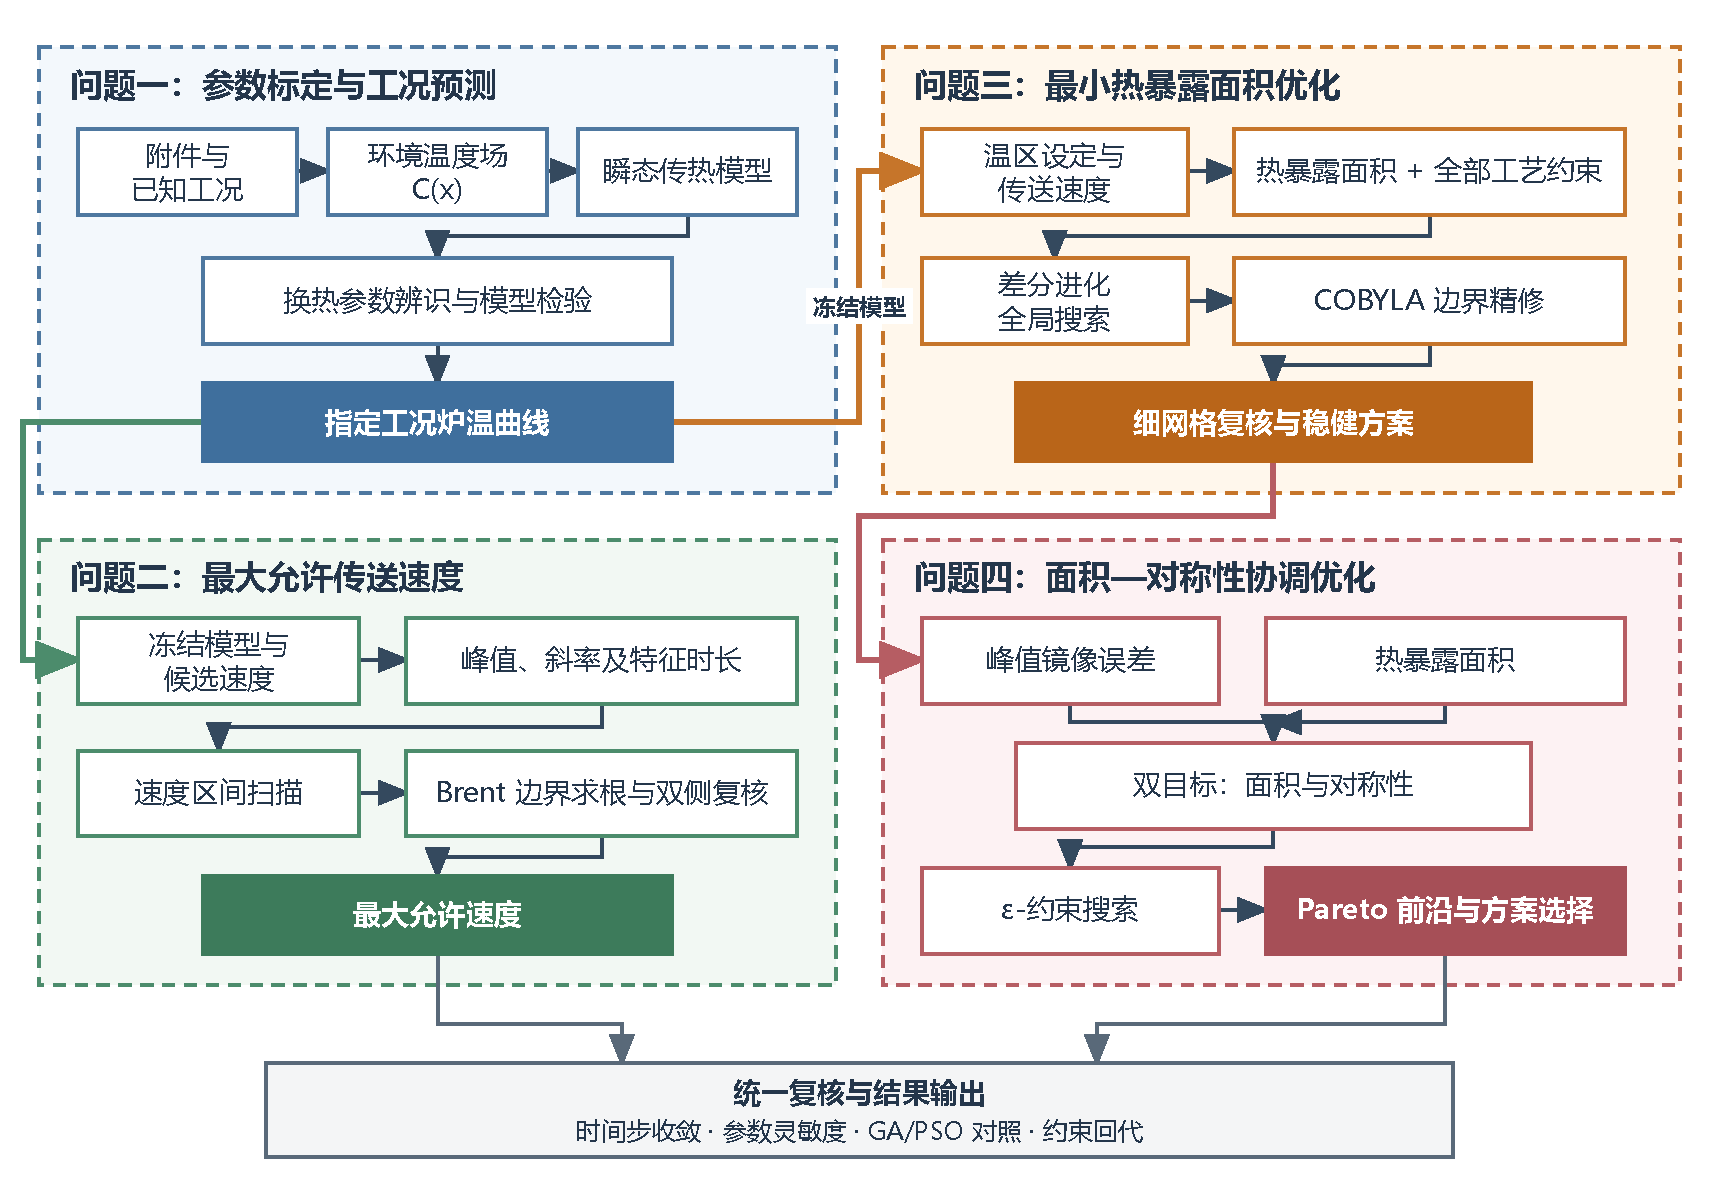
\includegraphics[width=0.98\textwidth]{paper/model_workflow.pdf}
  \caption{回焊炉炉温曲线建模与优化的总体工作流程}
  \label{fig:model-workflow}
\end{figure}

\subsection{问题一：由实验曲线反推传热参数}

温区设定值描述的是加热装置的控制目标，不是移动焊点的瞬时温度。建模需先回答两个问题：焊点沿炉膛移动时接触怎样的环境温度，环境热量又怎样传到焊接区域中心。为此将模型分成“空间温度场”和“板内传热”两层。前者处理炉口、温区和间隙，后者处理热惯性。附件数据用于辨识换热参数；完成辨识后把参数冻结，再代入问题一的新工况进行预测。

\subsection{问题二：寻找一维可行域的右端点}

温区设定固定后，只有速度 $v$ 需要确定。每给定一个速度，正向模型可产生一条炉温曲线，进而算出峰值、斜率和特征时长。因此问题二可转化为一维约束极值问题。先扫描速度区间以免漏掉不连续的可行段，再对发生符号变化的约束裕量求根，便能同时说明“最大值是多少”和“是哪一条约束限制了速度”。

\subsection{问题三：在可行域内压缩热暴露}

第三问同时调节四组温度和速度，目标又由阈值穿越和峰值位置共同决定，难以写出稳定的解析梯度。适合采用全局搜索找到可行盆地，再用无导数局部算法精修。由于最优解很可能落在工艺边界上，粗时间步造成的峰值误差会直接改变可行性，故搜索结果必须在更细网格上重新排序和复核。

\subsection{问题四：先给出前沿，再说明选择偏好}

“面积小”和“左右对称”是两个不同目标，不宜在没有说明量纲与权重时直接相加。先构造能够同时反映持续时间差和形状差的镜像误差，再用 $\varepsilon$-约束法生成 Pareto 解集。这样既能观察两目标的交换关系，也能在需要唯一工艺时依据明确偏好选择面积优先、均衡或对称优先方案。

\section{模型假设与符号说明}

\subsection{模型假设}

\begin{enumerate}[label=\textbf{H\arabic*.},leftmargin=3em,itemsep=2pt]
  \item 回焊炉在电路板进入前已稳定运行，故等效环境温度只随位置变化，记为 $C(x)$。
  \item 电路板匀速运动，位置与时间满足 $x(t)=vt/60$，其中 $v$ 的单位为 cm/min。
  \item 焊接区域厚度远小于炉膛纵向尺度，忽略板面内的温差，只考虑厚度方向导热；上下表面换热条件相同，温度场关于中面对称。
  \item 焊接区域的热物性在工作温度范围内视为常数，入炉时温度均为车间温度 $25\,\dC$。
  \item 电路板对炉内温度场的反作用可忽略；对流和辐射的综合作用并入分段等效换热参数。
  \item 受控温区内部的等效环境温度取设定值。普通间隙没有独立热源，其稳定温度由两侧温区共同决定，而不是重新回到车间温度 $25\,\dC$。
\end{enumerate}

最后一项区分了两个不同概念：$25\,\dC$ 是车间和进炉初始温度；炉内 $5\,$cm 间隙虽不控温，但在稳定运行时仍处在两侧热源形成的温度场中。只有题目明确规定的温区 10--11 才保持 $25\,\dC$。

\subsection{主要符号}

\begin{table}[htbp]
  \centering
  \caption{主要符号及含义}
  \label{tab:symbols}
  \small
  \begin{tabularx}{\textwidth}{cYcY}
    \toprule
    符号 & 含义 & 符号 & 含义 \\
    \midrule
    $x,t$ & 炉内位置/cm，时间/s & $v$ & 传送速度/(cm/min) \\
    $S_i$ & 第 $i$ 小温区设定温度/\dC & $C(x)$ & 等效环境温度/\dC \\
    $T(z,t)$ & 焊接区域内部温度/\dC & $T_c,T_s$ & 中心温度、表面温度/\dC \\
    $\delta$ & 焊接区域厚度，$0.15\,$mm & $\alpha$ & 热扩散率/(m$^2$/s) \\
    $\eta_j$ & 第 $j$ 段等效换热参数 $h_j/\lambda$ & $t_u,t_p,t_d$ & 上穿 $217\,\dC$、峰值、下穿时刻 \\
    $A_L,A_R$ & 峰值左、右侧超温面积 & $J_{\mathrm{sym}}$ & 峰值镜像对称指标 \\
    $g_j$ & 第 $j$ 项工艺约束裕量 & $\Delta t$ & 数值计算时间步长/s \\
    \bottomrule
  \end{tabularx}
\end{table}

\section{炉温曲线基础模型与问题一求解}

\subsection{炉体几何与运动关系}

炉体由炉前区、11 个小温区、10 个间隙和炉后区依次组成，总长为

\begin{equation}
  L=25+11\times30.5+10\times5+25=435.5\ \mathrm{cm}.
  \label{eq:len}
\end{equation}

第 $i$ 个小温区的起止位置为

\begin{equation}
  a_i=25+(i-1)(30.5+5),\qquad b_i=a_i+30.5,
  \quad i=1,\ldots,11.
\end{equation}

传送带匀速时，焊接区域的位置为 $x(t)=vt/60$。因此温区结构先在空间坐标 $x$ 下描述，再由该式转化为焊点随时间经历的外部热环境。图 \ref{fig:furnace} 同时给出炉体结构和标定工况下的等效环境温度场。

\begin{figure}[htbp]
  \centering
  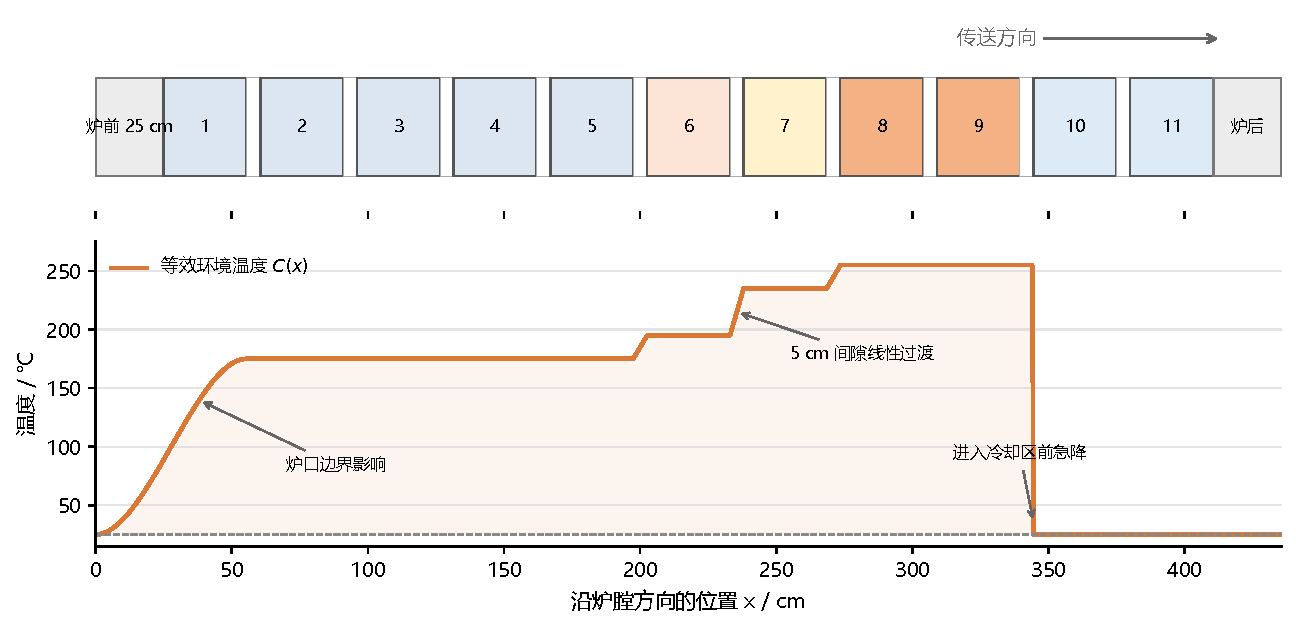
\includegraphics[width=0.96\textwidth]{paper/furnace_ambient.pdf}
  \caption{炉体结构及等效环境温度场示意}
  \label{fig:furnace}
\end{figure}

\subsection{等效环境温度场}
\label{sec:amb}

设 $C(x)$ 为焊接区域在位置 $x$ 处所感受到的等效环境温度。它不是焊点中心温度，而是后续传热方程的外部边界条件。受控温区、普通间隙和炉体两端的形成机理不同，需要分别处理。

\subsubsection{受控温区与普通间隙}

远离炉口和冷却入口时，第 $i$ 个受控温区内取 $C(x)=S_i$。相邻温区之间的 $5\,$cm 间隙没有独立热源；炉体稳定运行后，间隙内温度由两侧温区传热共同决定。在忽略横向散热且等效导热系数不变的一维近似下，间隙满足

\begin{equation}
  \frac{\mathrm d^2C}{\mathrm dx^2}=0.
\end{equation}

结合两端条件 $C(b_i)=S_i$、$C(a_{i+1})=S_{i+1}$，得到

\begin{equation}
  C(x)=S_i+\frac{S_{i+1}-S_i}{5}(x-b_i),
  \qquad b_i<x<a_{i+1}.
  \label{eq:gap}
\end{equation}

可见，间隙采用线性连接并非任意插值，而是无内热源稳态一维导热方程的解。这里也不应把间隙温度设为 $25\,\dC$：$25\,\dC$ 是车间温度和电路板初温，内部间隙在稳定炉膛内会持续受到两侧热区影响。

\subsubsection{炉口和冷却入口的边界影响}

若令炉前 $25\,$cm 直接线性升至 $S_1$，模型在实验曲线前段产生明显高估。这说明冷空气侵入的影响延伸到了第 1 温区内部。将炉口至第 1 区出口 $b_1=55.5\,$cm 作为有效入口段，并取

\begin{equation}
  H(s)=3s^2-2s^3,\qquad
  C(x)=25+(S_1-25)H\!\left(\frac{x}{b_1}\right),
  \quad 0\le x<b_1.
  \label{eq:front}
\end{equation}

$H(0)=0,H(1)=1$ 且 $H'(0)=H'(1)=0$，故入口温度及其梯度均连续。三次 Hermite 函数在此只承担边界连接作用，入口段长度则由炉体结构和残差比较确定；它并不是对焊点实测曲线的多项式拟合。

第 9 区后进入冷却区。为避免在边界处使用不符合实际的数学阶跃，令高温气流延续到第 10 区入口前 $w=0.5\,$cm，并在该短区间内由 Hermite 函数降至 $25\,\dC$：

\begin{equation}
  C(x)=
  \begin{cases}
    S_9, & b_9<x\le a_{10}-w,\\
    S_9+(25-S_9)H\!\left(\dfrac{x-a_{10}+w}{w}\right),
      &a_{10}-w<x<a_{10},\\
    25, &a_{10}\le x\le b_{11}.
  \end{cases}
  \label{eq:cool}
\end{equation}

对 $w=0.1\sim1.0\,$cm 的试算显示，RMSE 和峰值时刻的变化均很小，故取 $0.5\,$cm 作为有限宽度的代表值。式 \eqref{eq:gap}--\eqref{eq:cool} 与受控区常值共同组成连续的 $C(x)$。

\subsection{焊接区域的瞬态传热模型}

焊接区域厚度为 $\delta=0.15\,$mm，远小于沿炉膛方向的尺度。利用上下表面对称性，只计算中面到上表面的半厚度 $0\le z\le\delta/2$。一维非稳态导热方程为\cite{eftychiou1993}

\begin{equation}
  \frac{\partial T}{\partial t}
  =\alpha\frac{\partial^2T}{\partial z^2},
  \qquad 0<z<\frac{\delta}{2}.
  \label{eq:pde}
\end{equation}

中面对称条件、初始条件和表面换热条件分别为

\begin{equation}
  \left.\frac{\partial T}{\partial z}\right|_{z=0}=0,
  \qquad T(z,0)=25,
  \qquad
  \lambda\left.\frac{\partial T}{\partial z}\right|_{z=\delta/2}
  =h_j\,[C(x(t))-T_s].
  \label{eq:robin}
\end{equation}

式 \eqref{eq:robin} 表明，温区设定先形成外部温度 $C(x)$，再通过表面对流与辐射的综合换热使板面升温，最后由导热传到中心。这一过程自然产生炉温曲线相对环境温度场的滞后。模型中 $h_j$ 与导热系数 $\lambda$ 以组合形式出现，记

\begin{equation}
  \eta_j=\frac{h_j}{\lambda}.
\end{equation}

仅有一条中心温度曲线时，$h_j$、$\lambda$、热扩散率和辐射率无法同时稳定辨识。因此固定 $\alpha=1.5\times10^{-7}\,$m$^2$/s，把辐射贡献并入分段等效参数 $\eta_j$。回焊炉不同工艺区的换热条件存在显著差异，采用分区等效换热系数也与实测研究相符\cite{illes2010}。结合炉体工艺段和残差分布，将 $\eta$ 划分为表 \ref{tab:eta} 的五段。

\begin{table}[htbp]
  \centering
  \caption{分段等效换热参数及辨识结果}
  \label{tab:eta}
  \small
  \begin{tabular}{clcr}
    \toprule
    段 & 空间范围 & 参数 & 辨识值/m$^{-1}$ \\
    \midrule
    1 & 炉口至第 5 区出口 & $\eta_{\mathrm{pre}}$ & $9.4783$ \\
    2 & 第 6 区 & $\eta_{\mathrm{soak}}$ & $7.4014$ \\
    3 & 第 7 区至第 9 区出口 & $\eta_{\mathrm{ref}}$ & $11.0839$ \\
    4 & 第 9 区出口至第 10 区出口 & $\eta_{\mathrm{cool,1}}$ & $1.6029$ \\
    5 & 第 10 区出口以后 & $\eta_{\mathrm{cool,2}}$ & $4.7537$ \\
    \bottomrule
  \end{tabular}
\end{table}

\subsection{数值离散与参数辨识}

厚度方向取 11 个等距节点，时间方向采用隐式 Euler 离散。记 $r=\alpha\Delta t/\Delta z^2$，内部节点满足

\begin{equation}
  -r u_{k-1}^{n+1}+(1+2r)u_k^{n+1}-r u_{k+1}^{n+1}=u_k^n.
  \label{eq:implicit}
\end{equation}

中面条件用镜像节点处理，表面条件由一阶差分代入式 \eqref{eq:robin}。每个时间步均得到三对角线性方程组，采用 Thomas 追赶法求解\cite{patankar1980}。阈值温度的穿越时刻则在相邻时间节点间线性插值：

\begin{equation}
  t_{\mathrm{cross}}=t_k+
  \frac{\Theta-T_k}{T_{k+1}-T_k}(t_{k+1}-t_k).
  \label{eq:cross}
\end{equation}

用附件的 709 个观测点辨识五个 $\eta_j$，最小化目标为

\begin{equation}
  \min_{\bm\eta>0}\sum_{m=1}^{709}
  \left[T_c(t_m;\bm\eta)-T_m^{\mathrm{obs}}\right]^2.
  \label{eq:ls}
\end{equation}

采用有界信赖域反射算法并从三组初值出发。最终得到

\begin{equation}
  \mathrm{RMSE}=1.1197\,\dC,\qquad
  \mathrm{MAE}=0.7167\,\dC,\qquad
  \max|e|=4.0471\,\dC.
\end{equation}

图 \ref{fig:calib} 显示模型已消除基准模型在炉前和冷却后段的大范围系统偏差，但在回流和急冷转换附近仍存在局部结构性残差。这些局部误差提示等效温度场仍是炉内复杂流动的低维近似，后文将通过敏感性分析评估其影响。

\begin{figure}[htbp]
  \centering
  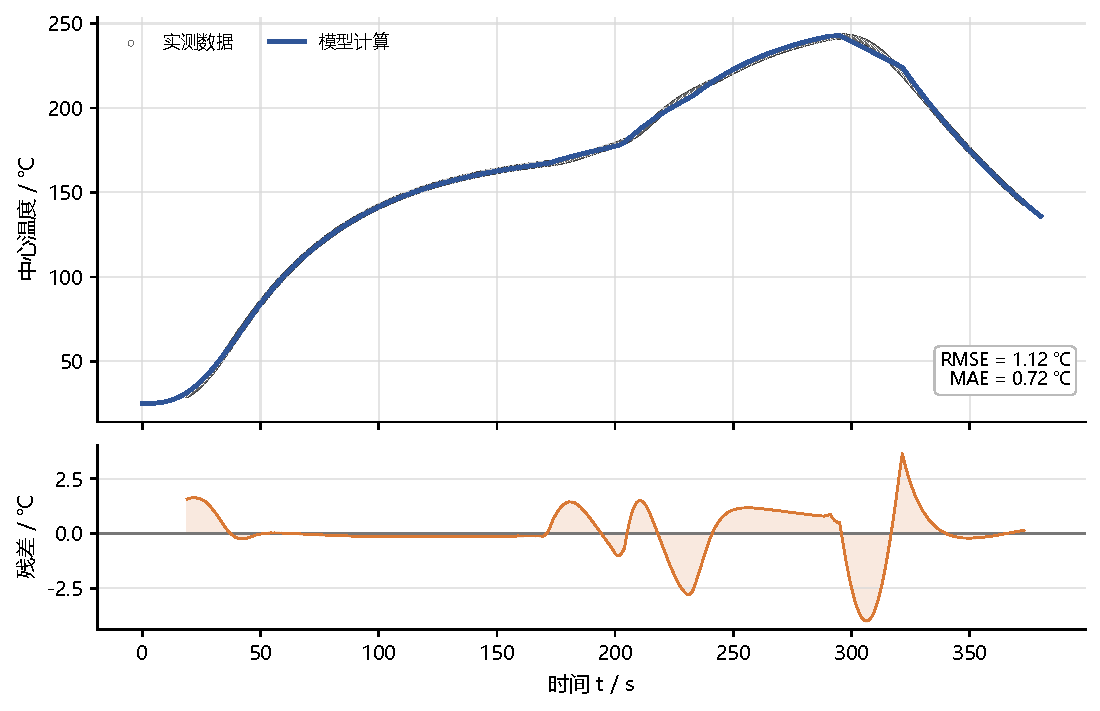
\includegraphics[width=0.82\textwidth]{paper/calibration_fit.pdf}
  \caption{标定工况下模型计算值、实测值及残差}
  \label{fig:calib}
\end{figure}

为防止增加参数后只获得表面上的拟合改善，进一步用 Jacobian 条件数衡量可辨识性。表 \ref{tab:candidates} 给出主要候选结构。C4 相对于 C3 将 RMSE 从 $2.0699\,\dC$ 降至 $1.9308\,\dC$，但条件数增至 $2.8\times10^8$，参数对数据扰动极为敏感；定稿模型则在更低 RMSE 下仍保持良好条件数。因此模型选择依据是“预测误差与参数稳定性同时可接受”，而不是一味增加自由参数。

\begin{table}[htbp]
  \centering
  \caption{主要候选模型的拟合与可辨识性比较}
  \label{tab:candidates}
  \small
  \begin{tabular}{lcrr}
    \toprule
    模型结构 & RMSE/\dC & AIC & $\kappa(\bm J)$ \\
    \midrule
    炉前线性、单冷却段（C0） & $6.9535$ & $2757.8$ & $2.3\times10^1$ \\
    加入口损失、双冷却段（C2） & $2.1930$ & $1125.5$ & $1.9\times10^5$ \\
    再拆分炉前换热（C4） & $1.9308$ & $949.0$ & $2.8\times10^8$ \\
    \textbf{Hermite 入口、五段换热（定稿）} & $\bm{1.1197}$ & $\bm{170.3}$ & $\bm{1.58\times10^1}$ \\
    \bottomrule
  \end{tabular}
\end{table}

\subsection{问题一结果}

辨识完成后固定表 \ref{tab:eta} 的参数，代入 $S_{1\text{-}5}=173\,\dC$、$S_6=198\,\dC$、$S_7=230\,\dC$、$S_{8\text{-}9}=257\,\dC$ 和 $v=78\,$cm/min。炉内总时间为 $335.0\,$s。四个指定位置由 $t=x/(v/60)$ 转换，对应中心温度见表 \ref{tab:q1probe}。

\begin{table}[htbp]
  \centering
  \caption{问题一指定位置的焊接区域中心温度}
  \label{tab:q1probe}
  \small
  \begin{tabular}{lrrr}
    \toprule
    位置 & $x$/cm & $t$/s & $T_c$/\dC \\
    \midrule
    小温区 3 中点 & $111.25$ & $85.5769$ & $\bm{131.15}$ \\
    小温区 6 中点 & $217.75$ & $167.5000$ & $\bm{169.36}$ \\
    小温区 7 中点 & $253.25$ & $194.8077$ & $\bm{189.28}$ \\
    小温区 8 出口 & $304.00$ & $233.8462$ & $\bm{225.68}$ \\
    \bottomrule
  \end{tabular}
\end{table}

完整炉温曲线如图 \ref{fig:q1prof}。其峰值为 $240.6257\,\dC$，最大升温速率为 $2.0538\,\dC$/s，最小降温速率为 $-1.9897\,\dC$/s；升温时处于 $150\sim190\,\dC$ 的时间为 $79.95\,$s，高于 $217\,\dC$ 的时间为 $68.7193\,$s。五项指标均满足表 \ref{tab:limits}。按题目要求，每隔 $0.5\,$s 的 671 行结果写入 \texttt{result.csv}。

\begin{figure}[htbp]
  \centering
  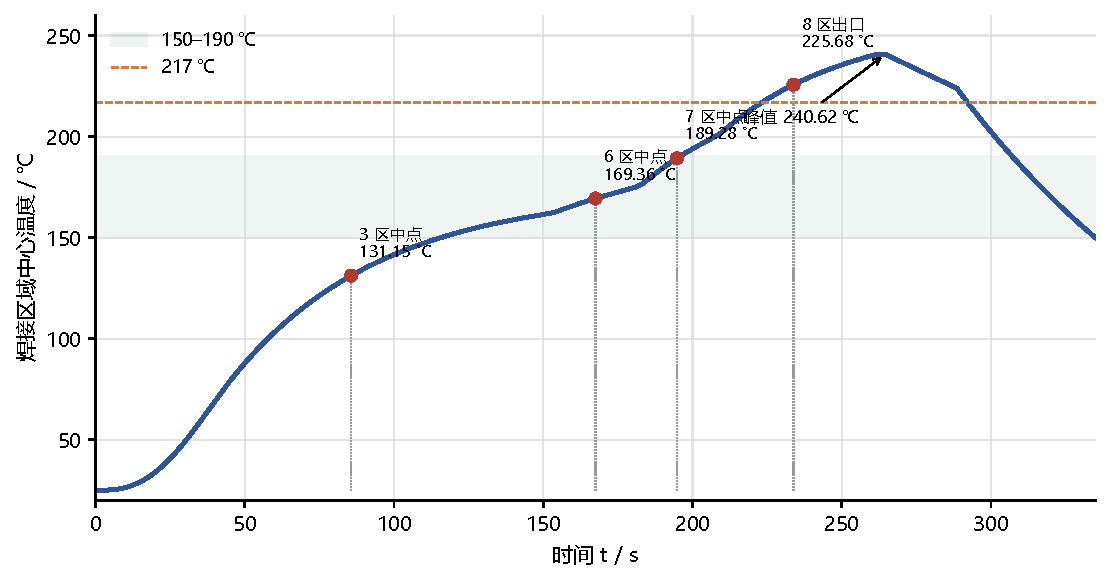
\includegraphics[width=0.84\textwidth]{paper/q1_profile.pdf}
  \caption{问题一工况下的炉温曲线及四个指定位置}
  \label{fig:q1prof}
\end{figure}

\section{问题二：最大允许过炉速度}

\subsection{约束模型}

本问四组温区设定依次为 $182\,\dC$、$203\,\dC$、$237\,\dC$ 和 $254\,\dC$。唯一决策变量是速度，其范围为 $65\sim100\,$cm/min。对每个候选速度调用上一节模型，得到峰值温度 $T_{\max}$、升降温速率、升温时处于 $150\sim190\,\dC$ 的时间 $\tau_{150-190}$ 以及高于 $217\,\dC$ 的时间 $\tau_{217}$。将表 \ref{tab:limits} 展开为十个非负裕量：

\begin{equation}
\begin{aligned}
  &g_1=3-r_{\mathrm{up}}^{\max}, &&g_2=r_{\mathrm{up}}^{\min}+\epsilon_0,
  &&g_3=r_{\mathrm{dn}}^{\min}+3, &&g_4=-r_{\mathrm{dn}}^{\max},\\
  &g_5=\tau_{150-190}-60, &&g_6=120-\tau_{150-190},
  &&g_7=\tau_{217}-40, &&g_8=90-\tau_{217},\\
  &g_9=T_{\max}-240, &&g_{10}=250-T_{\max}.&&&&
\end{aligned}
\label{eq:margins}
\end{equation}

其中 $\epsilon_0=10^{-3}\,\dC$/s 用于吸收恒温段接近零斜率时的数值扰动。若曲线未穿越某一阈值，则相应时长约束直接判为不满足。于是问题写成

\begin{equation}
  \max_{65\le v\le100}v,
  \qquad \text{s.t.}\quad g_j(v)\ge0,\ j=1,\ldots,10.
  \label{eq:q2}
\end{equation}

这里仍使用问题一辨识出的参数。速度只改变 $x(t)=vt/60$，不改变炉体本身；若随候选速度重新拟合换热参数，优化的将不再是同一台回焊炉。

\subsection{扫描、求根与边界复核}

虽然峰值温度随速度在本工况下近似单调下降，但所有工艺指标未必具有相同单调性，因此不直接对整个区间二分。具体步骤为：先以 $1\,$cm/min 扫描 $[65,100]$，记录每个 $g_j$ 的符号；再对出现符号变化的子区间用 Brent 法求解 $g_j(v)=0$；最后以所有根和扫描点划分子区间，在区间中点复核可行性。

得到三个边界根，见表 \ref{tab:roots}。其中 $g_8=0$ 决定可行域下界，$g_9=0$ 决定上界，而 $g_5=0$ 位于不可行区域，不能形成新的可行段。

\begin{table}[htbp]
  \centering
  \caption{问题二的约束边界}
  \label{tab:roots}
  \small
  \begin{tabular}{llrl}
    \toprule
    约束 & 物理含义 & 根/(cm/min) & 对可行域的作用 \\
    \midrule
    $g_8=0$ & 高于 $217\,\dC$ 的时间达到 $90\,$s & $68.0016$ & 下界 \\
    $g_9=0$ & 峰值温度降至 $240\,\dC$ & $79.5937$ & 上界 \\
    $g_5=0$ & $150\sim190\,\dC$ 时间降至 $60\,$s & $97.6745$ & 已在可行域外 \\
    \bottomrule
  \end{tabular}
\end{table}

连续速度上界为 $v^*=79.59363\,$cm/min。按 $0.01\,$cm/min 的报告精度向可行侧取值，得到

\begin{equation}
  \boxed{v_{\max}=79.60\ \mathrm{cm/min}}.
\end{equation}

该速度下峰值温度为 $240.00185\,\dC$，最大升温速率为 $2.19241\,\dC$/s，最小降温速率为 $-1.98717\,\dC$/s，$\tau_{150-190}=83.7863\,$s，$\tau_{217}=71.4307\,$s，均满足约束。进一步在同一时间网格上检验边界两侧：$79.60\,$cm/min 可行，而 $79.61\,$cm/min 时峰值降至 $239.99343\,\dC$，故 $79.60$ 确为报告精度下的最大可行速度。

图 \ref{fig:q2scan} 揭示了可行区间的形成过程。低速时板在高温区停留过久，先违反 $\tau_{217}\le90\,$s；速度提高后进入可行域；当速度超过 $79.59\,$cm/min，吸热时间不足，峰值又低于 $240\,\dC$。因此本问并不存在“速度越慢越安全”的单调关系。

\begin{figure}[htbp]
  \centering
  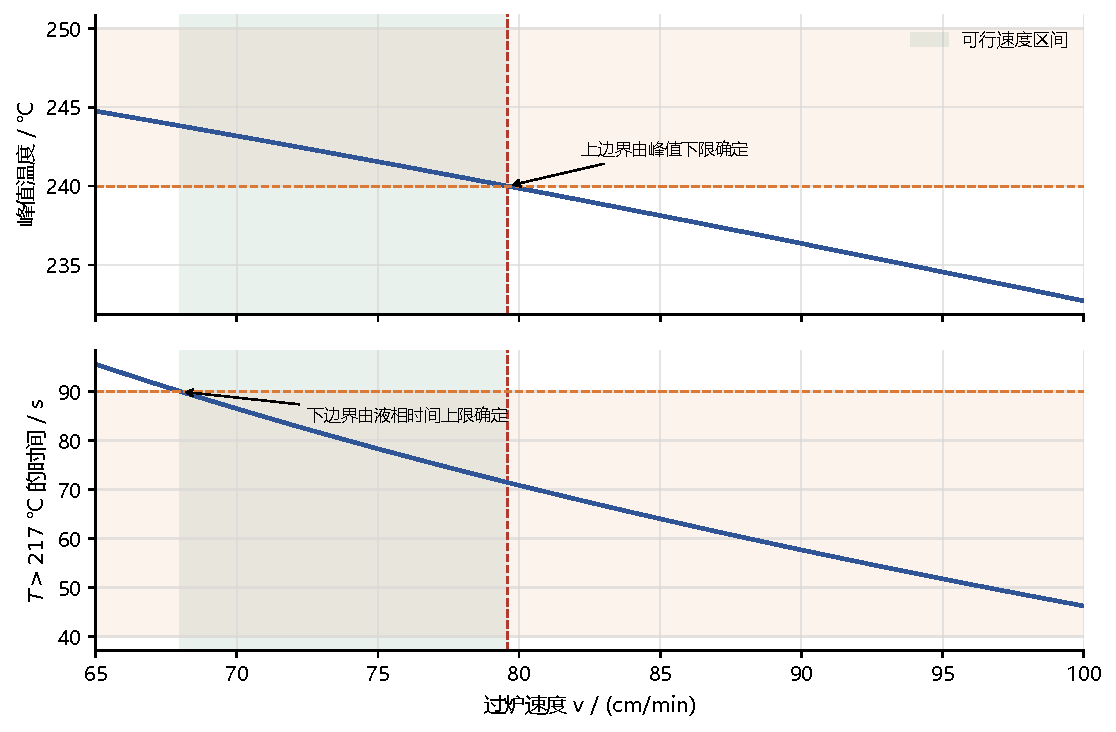
\includegraphics[width=0.84\textwidth]{paper/q2_constraint_boundary.pdf}
  \caption{峰值温度和液相线以上时间随速度的变化及可行区间}
  \label{fig:q2scan}
\end{figure}

\section{问题三：最小热暴露面积}

\subsection{目标函数与约束}

根据温区联动关系，取五维决策变量

\begin{equation}
  \bm y=(S_{1-5},S_6,S_7,S_{8-9},v)\in\Omega,
\end{equation}

其中

\begin{equation}
  \Omega=[165,185]\times[185,205]\times[225,245]
  \times[245,265]\times[65,100].
  \label{eq:omega}
\end{equation}

为避免温度和速度的量纲差异影响搜索，将每个变量线性映射到 $[0,1]$。记炉温曲线首次上穿 $217\,\dC$ 的时刻为 $t_u$，峰值时刻为 $t_p$。题目要求的阴影面积是升温侧超出液相线的面积，故目标函数为

\begin{equation}
  A(\bm y)=\int_{t_u}^{t_p}[T(t;\bm y)-217]\,\mathrm dt,
  \qquad \min_{\bm y\in\Omega}A(\bm y).
  \label{eq:q3obj}
\end{equation}

该面积同时反映液相线以上的温度和持续时间。数值积分前先按式 \eqref{eq:cross} 插值得到 $t_u$，再把 $t_u$ 和 $t_p$ 插入积分节点，用梯形公式计算，避免阈值端点落在两个时间节点之间造成固定偏差。

约束仍为式 \eqref{eq:margins} 的十个工艺裕量。为比较不同单位的违反程度，令 $c_j=-g_j$，定义

\begin{equation}
  V(\bm y)=\sum_{j=1}^{10}\max\left(0,\frac{c_j(\bm y)}{s_j}\right),
  \quad
  \bm s=(3,3,3,3,60,60,50,50,10,10).
  \label{eq:V}
\end{equation}

搜索时采用 Deb 可行性规则\cite{deb2000}：可行解优于不可行解；两个可行解比较面积；两个不可行解比较 $V$。这样无需人为选择罚函数系数。

\subsection{全局搜索与边界精修}

目标函数包含 PDE 仿真、阈值穿越、峰值和最大斜率运算，随参数变化呈分段光滑，直接使用解析梯度容易在事件点失效。本文采用两阶段求解：

\begin{enumerate}[label=\textbf{步骤\arabic*.},leftmargin=3.7em,itemsep=2pt]
  \item 用拉丁超立方产生初始种群，并加入问题二的可行工艺作为种子；采用差分进化的 rand/1 变异和二项交叉进行全局探索\cite{storn1997}，选择阶段执行 Deb 规则。
  \item 从种群中选取空间上分散的可行精英，以其为起点运行 COBYLA\cite{powell1994}，在不求导的条件下细化目标和约束边界。
\end{enumerate}

计算精度与优化过程同时控制。全局搜索先在 $\Delta t=0.1\,$s 网格上进行；精英在 $0.05\,$s 网格上重新评价和排序；最终在 $0.025\,$s 网格上再次精修，并只接受此时仍满足全部约束的解。这里的“重新排序”很重要：最优解紧贴峰值下限，粗网格约 $0.1\,\dC$ 的峰值误差足以改变可行性，不能把粗网格排名直接沿用到最终结果。

\subsection{最小面积解及其形成机理}

在 $\Delta t=0.025\,$s 网格上得到的最优可行结果见表 \ref{tab:q3opt}，目标值为

\begin{equation}
  \boxed{A^*=410.680629\ \dC\!\cdot\!\mathrm s}.
\end{equation}

\begin{table}[htbp]
  \centering
  \caption{问题三最小面积解}
  \label{tab:q3opt}
  \small
  \begin{tabular}{lr@{\qquad}lr}
    \toprule
    工艺参数 & 数值 & 炉温曲线指标 & 数值 \\
    \midrule
    $S_{1-5}$/\dC & $184.9996$ & 峰值温度/\dC & $240.000001$ \\
    $S_6$/\dC & $198.2817$ & 最大升温速率/(\dC/s) & $2.37987$ \\
    $S_7$/\dC & $238.0047$ & 最小降温速率/(\dC/s) & $-2.01852$ \\
    $S_{8-9}$/\dC & $265.0000$ & $\tau_{150-190}$/s & $61.13214$ \\
    $v$/(cm/min) & $99.5068$ & $\tau_{217}$/s & $54.03496$ \\
    \bottomrule
  \end{tabular}
\end{table}

图 \ref{fig:q3curve} 给出目标面积。该解的结构并非偶然：$S_{1-5}$ 和 $S_{8-9}$ 到达上界，速度接近上界，而峰值恰好落在 $240\,\dC$ 下限。提高前段温度使焊点在进入回流区前已有较高温度，缩短从 $217\,\dC$ 升至峰值的时间；提高速度进一步压缩高温停留；峰值若继续升高则会直接增加面积。因此目标下降方向最终被峰值下限封住。

\begin{figure}[htbp]
  \centering
  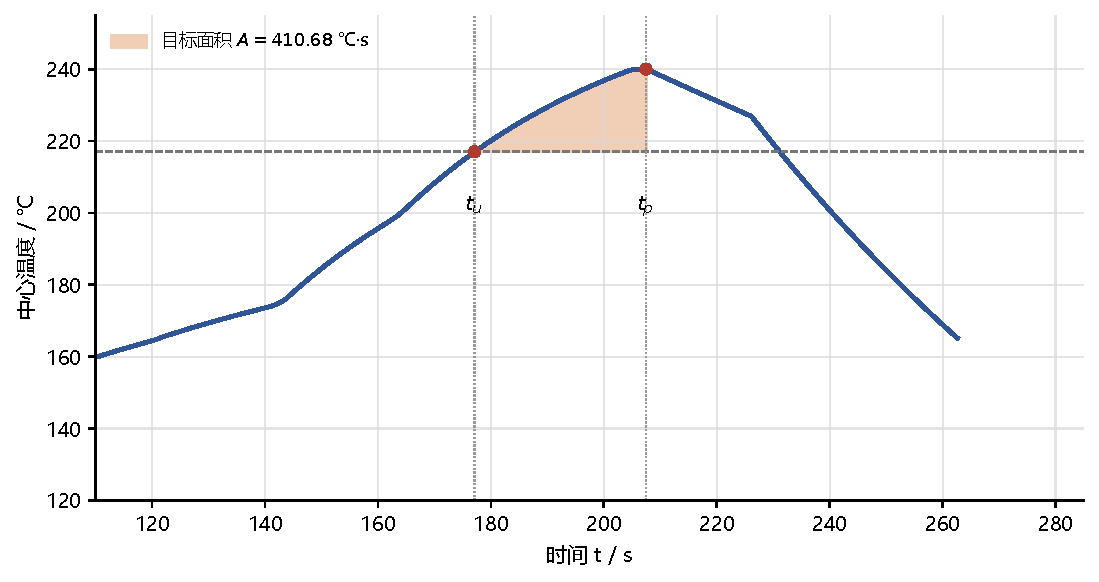
\includegraphics[width=0.82\textwidth]{paper/q3_area.pdf}
  \caption{问题三最优炉温曲线及目标面积}
  \label{fig:q3curve}
\end{figure}

为检查这一边界结构，对五个变量分别作温度 $\pm1\,\dC$、速度 $\pm0.5\,$cm/min 的单变量扰动。降低 $S_{1-5}$、$S_6$、$S_7$ 或 $S_{8-9}$，以及提高速度，都会使面积下降，但同时使峰值跌破 $240\,\dC$；其余保持可行的方向均使面积增加。该结果说明在所检验邻域内不存在可行的单变量下降方向。由于全局算法预算有限，本文将 $A^*$ 表述为“搜索并精修得到的最优可行值”，而不把随机搜索结果当作严格的全局最优证明。

\subsection{工程余量方案}

数学最优解的峰值裕量仅 $1.3\times10^{-6}\,\dC$，明显小于模型 RMSE 和实际温控波动，不能直接作为生产设定。为给出可实施方案，在原工艺约束之外加入

\begin{equation}
  T_{\max}\ge241\,\dC,\qquad
  \tau_{150-190}\ge62\ \mathrm s,\qquad
  \tau_{217}\ge42\ \mathrm s,
\end{equation}

并用同一算法重新优化，结果见表 \ref{tab:q3eng}。

\begin{table}[htbp]
  \centering
  \caption{理论最小面积解与工程余量方案}
  \label{tab:q3eng}
  \small
  \begin{tabular}{lrr}
    \toprule
    指标 & 最小面积解 & 工程余量方案 \\
    \midrule
    温区设定/\dC
      & \shortstack{$185.000/198.282$\\$238.005/265.000$}
      & \shortstack{$184.995/196.891$\\$241.766/264.998$} \\
    $v$/(cm/min) & $99.5068$ & $98.1524$ \\
    $A$/(\dC$\cdot$s) & $410.6806$ & $454.7800$ \\
    峰值温度/\dC & $240.0000$ & $241.0018$ \\
    参数单因素 $\pm5\%$ 扰动下可行数 & $6/10$ & $8/10$ \\
    \bottomrule
  \end{tabular}
\end{table}

工程方案以 $10.74\%$ 的面积增加换得更大的峰值和特征时长余量。前者回答题目中的数学最优，后者用于说明实际投产时应为模型误差和设备波动预留空间。

\section{问题四：面积与对称性的协调优化}

\subsection{峰值镜像对称指标}

第三问只考虑峰值左侧面积。第四问又要求高于 $217\,\dC$ 的左右两段尽量以峰值时刻为中心对称。记上穿、峰值和下穿 $217\,\dC$ 的时刻分别为 $t_u,t_p,t_d$，并定义

\begin{equation}
  A_L=\int_{t_u}^{t_p}[T(t)-217]\,\mathrm dt,
  \qquad
  A_R=\int_{t_p}^{t_d}[T(t)-217]\,\mathrm dt.
\end{equation}

将峰值两侧按到峰值的时间距离 $\tau$ 对齐：

\begin{equation}
\begin{aligned}
  q_L(\tau)&=\max\{T(t_p-\tau)-217,0\},\\
  q_R(\tau)&=\max\{T(t_p+\tau)-217,0\}.
\end{aligned}
\end{equation}

左右液相时长分别为 $\tau_L=t_p-t_u$、$\tau_R=t_d-t_p$。在较短一侧结束后补零，积分到 $\tau_{\max}=\max(\tau_L,\tau_R)$，得到镜像误差

\begin{equation}
  E_{\mathrm{sym}}=\int_0^{\tau_{\max}}
  |q_L(\tau)-q_R(\tau)|\,\mathrm d\tau.
  \label{eq:esym}
\end{equation}

因此，左右持续时间不同会形成补零区域，曲线形状不同会形成重叠区内的面积差，两类不对称均被计入。

若用 $A_L+A_R$ 作为分母，优化器可能通过提高峰值或延长液相时间扩大分母，从而在绝对误差没有改善时仍使比值减小。为避免这一现象，采用由题目上限确定且与候选解无关的固定尺度

\begin{equation}
  S_0=(250-217)\times90=2970\ \dC\!\cdot\!\mathrm s,
  \qquad
  J_{\mathrm{sym}}=\frac{E_{\mathrm{sym}}}{S_0}.
  \label{eq:jsym}
\end{equation}

$J_{\mathrm{sym}}=0$ 对应完全对称，数值越小越好。固定正比例缩放不会改变最优解，同时保证不同工艺之间可以直接比较。

\subsection{约束法求解双目标模型}

问题四写成双目标约束优化：

\begin{equation}
  \min_{\bm y\in\Omega}\big(A_L(\bm y),J_{\mathrm{sym}}(\bm y)\big),
  \qquad \text{s.t.}\quad g_j(\bm y)\ge0.
  \label{eq:q4}
\end{equation}

若直接把两个目标线性加权，不仅需要预先规定权重，而且对非凸前沿的内部非支撑解可能搜索不到\cite{miettinen1998}。本文把面积转化为上限约束：

\begin{equation}
  \min_{\bm y}J_{\mathrm{sym}}(\bm y),
  \qquad
  \text{s.t.}\quad A_L(\bm y)\le\varepsilon_A,quad g_j(\bm y)\ge0.
  \label{eq:eps}
\end{equation}

令 $\varepsilon_A$ 从问题三最小面积逐步增加。

每个子问题仍采用差分进化和多起点 COBYLA，并在 $\Delta t=0.025\,$s 网格上统一复核。问题三的最优解自然成为该 Pareto 前沿的面积端点。

\subsection{Pareto 结果与方案选择}

严格非支配筛选得到 6 个点。其中两个点相对于面积端点的对称性改善仅为 $3.8\times10^{-4}$ 和 $4.0\times10^{-4}$，与时间离散带来的 $J_{\mathrm{sym}}$ 误差同量级。采用 $5\times10^{-4}$ 的数值分辨阈值后，保留表 \ref{tab:front} 的三个实用方案。其余精确点仍保存在结果文件中，但不据此作超出数值精度的工艺判断。

\begin{table}[htbp]
  \centering
  \caption{面积--对称性实用 Pareto 方案}
  \label{tab:front}
  \small
  \begin{tabular}{clrrr}
    \toprule
    方案 & 定位 & $A_L$/(\dC$\cdot$s) & $J_{\mathrm{sym}}$ & $v$/(cm/min) \\
    \midrule
    P1 & 面积最小（问题三解） & $410.6806$ & $0.0266313$ & $99.5068$ \\
    P4 & 均衡备选 & $415.7154$ & $0.0260712$ & $94.5129$ \\
    P6 & 对称优先 & $418.1586$ & $0.0248698$ & $89.6887$ \\
    \bottomrule
  \end{tabular}
\end{table}

从图 \ref{fig:q4} 左侧可见，实用前沿在目标空间中向远离理想点的一侧内凹，不存在稳定的几何膝点；这也意味着线性加权和无法生成该前沿上的内部支撑解。因此不能声称某个中间点是与偏好无关的“唯一最佳折中”。

若把两个目标的端点极差分别归一化后等权比较，可选 P4 作为均衡方案。考虑到第四问是在第三问基础上专门增加对称性要求，而 P6 相对于 P1 只增加 $1.82\%$ 面积，却使 $J_{\mathrm{sym}}$ 下降 $6.61\%$，本文把 P6 作为对称优先推荐解，同时保留 P4 供更强调热暴露的场景选择。P6 的参数见表 \ref{tab:q4final}。

\begin{table}[htbp]
  \centering
  \caption{问题四对称优先推荐方案}
  \label{tab:q4final}
  \small
  \begin{tabular}{lr@{\qquad}lr}
    \toprule
    工艺参数 & 数值 & 炉温曲线指标 & 数值 \\
    \midrule
    $S_{1-5}$/\dC & $171.3952$ & $A_L$/(\dC$\cdot$s) & $418.1586$ \\
    $S_6$/\dC & $188.9400$ & $A_R$/(\dC$\cdot$s) & $344.2953$ \\
    $S_7$/\dC & $226.3711$ & $E_{\mathrm{sym}}$/(\dC$\cdot$s) & $73.8633$ \\
    $S_{8-9}$/\dC & $264.9448$ & $J_{\mathrm{sym}}$ & $0.0248698$ \\
    $v$/(cm/min) & $89.6887$ & 峰值温度/\dC & $240.0109$ \\
    \midrule
    $\tau_L$/s & $30.6882$ & $\tau_R$/s & $25.0382$ \\
    $\tau_{150-190}$/s & $63.6662$ & $\tau_{217}$/s & $55.7264$ \\
    \bottomrule
  \end{tabular}
\end{table}

图 \ref{fig:q4} 右侧将推荐曲线沿峰值时刻对折。左右曲线形状相近，但升温侧持续时间仍比降温侧长约 $5.65\,$s。其原因是温区 10--11 固定在 $25\,\dC$，冷却段换热参数也不是决策变量，下降侧的宽度不能像前段温度和速度那样自由调节。因此推荐方案是现有控制变量下的最优协调，而不是严格的镜面对称。

\begin{figure}[htbp]
  \centering
  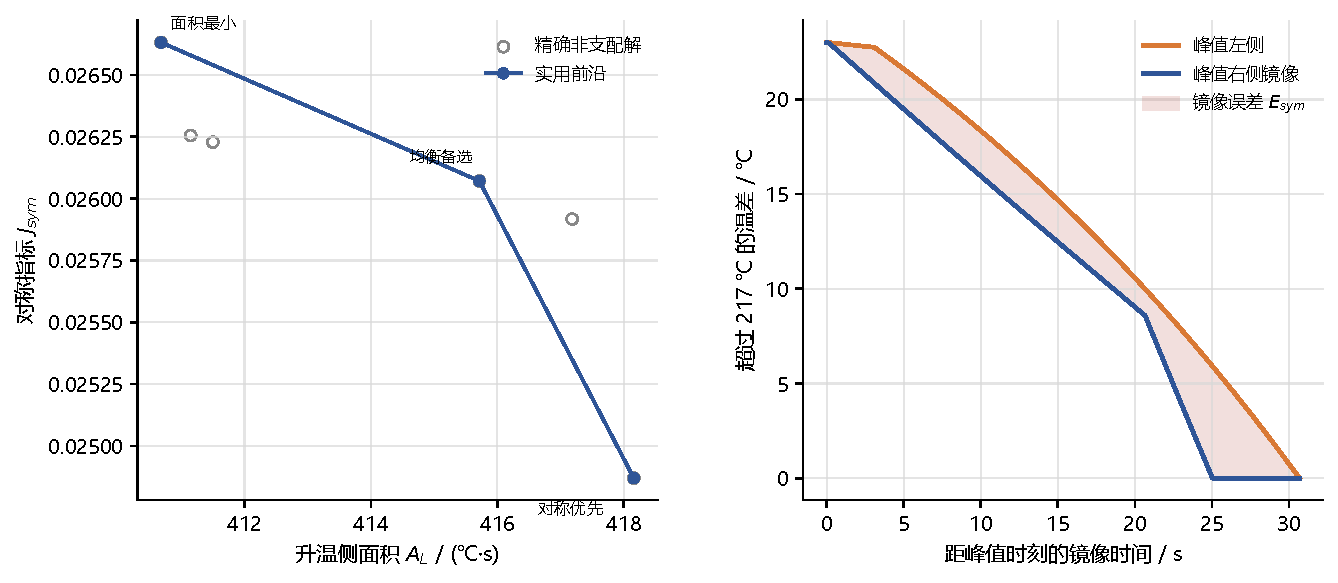
\includegraphics[width=0.96\textwidth]{paper/q4_tradeoff_mirror.pdf}
  \caption{问题四的面积--对称性前沿（左）与推荐解峰值镜像（右）}
  \label{fig:q4}
\end{figure}

\section{模型检验}

\subsection{时间步收敛性}
\label{sec:grid}

固定各问已得到的工艺参数，只改变时间步长重新计算关键结果，见表 \ref{tab:grid}。问题一指定位置温度在 $\Delta t\le0.05\,$s 后已稳定；问题二在 $0.025$ 和 $0.0125\,$s 网格上均报告 $79.60\,$cm/min；问题三面积的相对差为 $0.083\%$。因此以 $0.025\,$s 作为全文最终报告网格，可以兼顾边界判定精度与优化计算量。

\begin{table}[htbp]
  \centering
  \caption{关键结果的时间步收敛性}
  \label{tab:grid}
  \small
  \begin{tabular}{crrrcc}
    \toprule
    $\Delta t$/s & 问题一 3 区中点/\dC & 问题二 $v_{\max}$ & 问题三 $A$ & 问题三可行 & 问题四 $J_{\mathrm{sym}}$ \\
    \midrule
    $0.20$   & $131.1306$ & $79.38$ & $408.4327$ & 否 & $0.0228031$ \\
    $0.10$   & $131.1408$ & $79.53$ & $408.6284$ & 否 & $0.0236606$ \\
    $0.05$   & $131.1459$ & $79.58$ & $409.9962$ & 否 & $0.0241783$ \\
    $\bm{0.025}$ & $\bm{131.1484}$ & $\bm{79.60}$ & $\bm{410.6806}$ & 是 & $\bm{0.0248698}$ \\
    $0.0125$ & $131.1497$ & $79.60$ & $411.0229$ & 是 & $0.0247551$ \\
    \bottomrule
  \end{tabular}
\end{table}

表中还说明了三级网格的必要性。同一组问题三参数在 $0.10$ 和 $0.05\,$s 网格上会被判为不可行，而在细网格上满足约束。这不是物理状态改变，而是最优点的峰值裕量极小，离散峰值误差足以改变约束符号。粗网格适合搜索候选区域，最终可行性必须在细网格上重新判断。

\subsection{参数敏感性与工程余量}
\label{sec:sens}

对五个等效换热参数分别作 $\pm5\%$ 单因素扰动，共 10 种情形。图 \ref{fig:sens} 给出问题三面积的变化。回流段参数 $\eta_{\mathrm{ref}}$ 最敏感，$\pm5\%$ 扰动使面积约变化 $\pm47\,\dC\!\cdot\!\mathrm s$，峰值约变化 $\pm1.5\,\dC$；预热段次之。冷却段参数对 $A_L$ 几乎没有影响，因为第三问面积只积分到峰值，冷却发生在积分区间之后。这一结果与模型的因果顺序一致。

\begin{figure}[htbp]
  \centering
  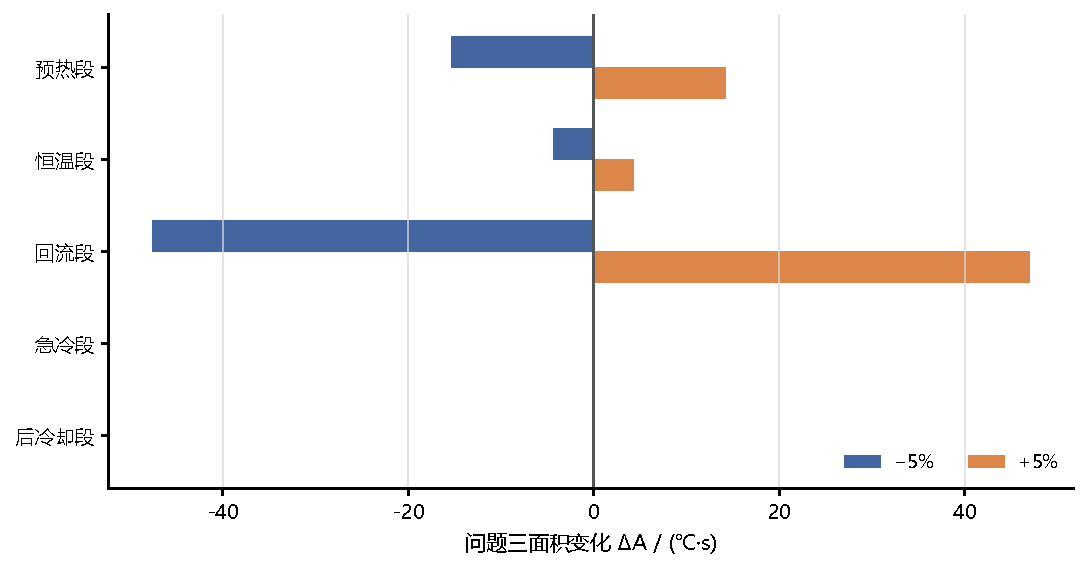
\includegraphics[width=0.78\textwidth]{paper/parameter_sensitivity.pdf}
  \caption{等效换热参数单因素扰动对问题三面积的影响}
  \label{fig:sens}
\end{figure}

参数减小往往使峰值跌破 $240\,\dC$。理论最小面积解在 10 种扰动下保持可行 6 次，工程余量方案保持可行 8 次，说明增加余量确实提高了稳健性，但尚不能替代多工况实验标定和更完整的不确定性分析。

\subsection{优化算法对照}
\label{sec:algo}

在相同种群规模、仿真预算、初始采样和 COBYLA 精修条件下，对差分进化、实数编码遗传算法和粒子群算法各进行一轮交叉检查，并统一在 $0.025\,$s 网格上复核。结果见表 \ref{tab:algo}。

\begin{table}[htbp]
  \centering
  \caption{三种全局搜索算法的同预算对照}
  \label{tab:algo}
  \small
  \begin{tabular}{lrrc}
    \toprule
    算法 & 最优可行面积/(\dC$\cdot$s) & 运行时间/s & 细网格可行 \\
    \midrule
    约束差分进化 $+$ COBYLA & $411.027$ & $183.4$ & 是 \\
    粒子群 $+$ COBYLA & $412.894$ & $177.8$ & 是 \\
    遗传算法 $+$ COBYLA & $424.780$ & $190.4$ & 是 \\
    \bottomrule
  \end{tabular}
\end{table}

三种方法均找到可行解，差分进化给出的面积最小；在其结果上继续高精度精修后得到正文的 $410.6806\,\dC\!\cdot\!\mathrm s$。由于这里只进行了单轮同预算比较，表 \ref{tab:algo} 用于说明主算法选择是经过交叉检查的，不能据此推断差分进化在所有类似问题中都优于另外两种算法。

\subsection{独立模型互校}

焊接区域很薄，中心与表面温差应当较小。为检查 PDE 离散实现，另建立集中参数模型

\begin{equation}
  \frac{\mathrm dT}{\mathrm dt}=k_j[C(x(t))-T]
  \label{eq:lumped}
\end{equation}

并用四阶 Runge--Kutta 独立求解。两种模型在标定工况下的最大温差为 $0.0614\,\dC$，问题一四个指定位置的差异均不超过 $0.02\,\dC$。两条不同的数值路径得到一致结果，既验证了程序实现，也说明对本题的薄焊接区域，厚度方向温差确实很小。

\section{模型评价}

\subsection{模型特点}

第一，模型把炉膛空间温度场与焊接区域热响应分开。速度只改变位置--时间映射，换热参数在标定后保持不变，因此四问比较的是同一台炉子上的不同工艺，而不是随候选解改变的模型。

第二，关键结构均有明确来源。普通间隙的线性温度来自无热源稳态导热方程；炉口和冷却入口的 Hermite 函数只用于保证边界值与梯度连续；板内温度来自非稳态导热方程和 Robin 边界。候选模型又通过拟合误差和 Jacobian 条件数共同筛选，避免用不可辨识的额外参数换取有限的残差下降。

第三，算法与问题结构相匹配。问题二是一维边界问题，使用扫描和求根能给出确定的双侧证据；问题三、四才使用群体搜索，并以局部精修、细网格复核和算法对照补强结果。对理论最优解和工程余量方案分别报告，也区分了数学目标与实际投产需求。

\subsection{模型局限}

等效环境温度场 $C(x)$ 没有直接求解炉内气流和辐射场，炉口影响长度及急冷宽度仍属于低维等效描述；若能获得 CFD 结果或炉内多点温度，可进一步确定这些空间结构。现有参数只由一条中心温度曲线标定，对流、辐射和材料物性不能分别辨识，局部残差也表明回流与急冷转换仍有改进空间。

模型忽略了板面方向的温差和元件热容差异。对尺寸较大、铜层分布不均或元件热容差别显著的电路板，应扩展为二维或三维传热模型。问题三最优点紧贴峰值下限，对模型误差敏感；工程余量方案虽改善单因素扰动下的可行率，但更完整的做法应是利用多工况数据建立参数分布，再进行鲁棒优化或机会约束优化。

多目标结论还依赖对称性的定义和生产偏好。本文的镜像误差兼顾持续时间与形状，但若企业更关注热应力，可进一步提高斜率差的权重。Pareto 前沿的部分细小改善已接近离散误差，因此没有把这些数值差异解释为真实工艺收益。

\section{结论}

本文以同一套“等效环境温度场--瞬态导热”模型贯穿四问。主要结果汇总于表 \ref{tab:final}。

\begin{table}[htbp]
  \centering
  \caption{四问主要结果}
  \label{tab:final}
  \footnotesize
  \begin{tabularx}{\textwidth}{c>{\raggedright\arraybackslash}p{5.8cm}Y}
    \toprule
    问题 & 工艺参数 & 主要结论 \\
    \midrule
    一 & 温区 $173/198/230/257\,\dC$，$v=78\,$cm/min（均为给定）
      & 四点温度为 $131.15,169.36,189.28,225.68\,\dC$；峰值 $240.63\,\dC$，工艺指标均合格。 \\
    二 & 温区 $182/203/237/254\,\dC$（给定），$\bm{v=79.60}\,$cm/min
      & 连续上界 $79.5936$；上界由峰值下限控制，可行区间约为 $[68.00,79.59]$。 \\
    三 & \shortstack[l]{温区 $185.000/198.282\,\dC$\\$238.005/265.000\,\dC$\\$v=99.5068\,$cm/min}
      & 最小升温侧面积 $\bm{410.6806\,\dC\!\cdot\!\mathrm s}$；另给出留有峰值余量的工程方案。 \\
    四 & \shortstack[l]{温区 $171.395/188.940\,\dC$\\$226.371/264.945\,\dC$\\$v=89.6887\,$cm/min}
      & 对称优先方案 $A_L=418.1586\,\dC\!\cdot\!\mathrm s$，$\bm{J_{\mathrm{sym}}=0.024870}$。 \\
    \bottomrule
  \end{tabularx}
\end{table}

问题一表明，炉内未控温间隙不应简单视为 $25\,\dC$，而应由稳定炉膛中两侧温区共同决定；焊点中心温度则由外部温度场经过传热滞后形成。问题二进一步说明最大速度不是由斜率限制，而是由吸热时间不足导致的峰值下限控制。问题三的面积最优点落在峰值约束边界，反映出“提高预热、缩短停留、压低峰值”的共同作用。问题四没有与偏好无关的唯一折中点，因此给出完整实用前沿，并在明确强调对称性的条件下选择推荐方案。

\begin{thebibliography}{99}
\addcontentsline{toc}{section}{参考文献}
\footnotesize

\bibitem{eftychiou1993}
Eftychiou M A, Bergman T L, Masada G Y. A Detailed Thermal Model of the Infrared Reflow Soldering Process[J]. Journal of Electronic Packaging, 1993, 115(1): 55--62.

\bibitem{illes2010}
Ill\'{e}s B. Measuring heat transfer coefficient in convection reflow ovens[J]. Measurement, 2010, 43(9): 1134--1141.

\bibitem{patankar1980}
Patankar S V. Numerical Heat Transfer and Fluid Flow[M]. New York: Hemisphere Publishing, 1980.

\bibitem{storn1997}
Storn R, Price K. Differential Evolution---A Simple and Efficient Heuristic for Global Optimization over Continuous Spaces[J]. Journal of Global Optimization, 1997, 11(4): 341--359.

\bibitem{deb2000}
Deb K. An efficient constraint handling method for genetic algorithms[J]. Computer Methods in Applied Mechanics and Engineering, 2000, 186(2--4): 311--338.

\bibitem{powell1994}
Powell M J D. A Direct Search Optimization Method That Models the Objective and Constraint Functions by Linear Interpolation[M]. Advances in Optimization and Numerical Analysis. Dordrecht: Springer, 1994: 51--67.

\bibitem{miettinen1998}
Miettinen K. Nonlinear Multiobjective Optimization[M]. Boston: Kluwer Academic Publishers, 1998.

\end{thebibliography}

\appendix
\addcontentsline{toc}{section}{附录}

\section{核心程序}

以下代码直接节选自实际运行的四个主程序，只保留环境温度场、隐式导热、约束边界、面积目标、差分进化和对称指标等决定结果的部分。绘图、命令行参数和文件写入不再重复列出，完整程序仍随论文文件一并提交。

\lstset{
  language=Python,
  basicstyle=\ttfamily\fontsize{7}{8}\selectfont,
  columns=fullflexible,
  keepspaces=true,
  tabsize=4,
  numbers=none,
  captionpos=t,
  aboveskip=6pt,
  belowskip=8pt
}

\lstinputlisting[firstline=105,lastline=132,caption={等效环境温度场的边界平滑（\texttt{q1.py}）}]{../code/q1.py}

\lstinputlisting[firstline=233,lastline=302,caption={半厚度一维非稳态导热的隐式求解（\texttt{q1.py}）}]{../code/q1.py}

\lstinputlisting[firstline=143,lastline=230,caption={约束边界定位与最大可行速度提取（\texttt{q2.py}）}]{../code/q2.py}

\lstinputlisting[firstline=145,lastline=167,caption={液相线以上升温侧面积计算（\texttt{q3.py}）}]{../code/q3.py}

\lstinputlisting[firstline=296,lastline=372,caption={Deb 规则与约束差分进化主循环（\texttt{q3.py}）}]{../code/q3.py}

\lstinputlisting[firstline=65,lastline=142,caption={固定尺度归一化的镜像对称指标（\texttt{q4.py}）}]{../code/q4.py}

\section{程序与结果文件}

主程序及辅助程序的作用见表 \ref{tab:code}。

\begin{table}[htbp]
  \centering
  \caption{程序文件及功能}
  \label{tab:code}
  \footnotesize
  \begin{tabularx}{\textwidth}{>{\raggedright\arraybackslash}p{5.2cm}Y}
    \toprule
    文件 & 功能 \\
    \midrule
    \texttt{code/q1.py} & 等效环境温度场、瞬态导热求解、参数辨识和问题一预测 \\
    \texttt{code/q2.py} & 工艺指标计算、速度扫描、Brent 边界求根 \\
    \texttt{code/q3.py} & 面积目标、约束差分进化、COBYLA 精修及算法对照 \\
    \texttt{code/q4.py} & 镜像误差、$\varepsilon$-约束子问题及 Pareto 筛选 \\
    \texttt{code/finalize\_results.py} & 统一细网格复算、时间步与参数敏感性检验 \\
    \texttt{code/closeout\_fix.py} & 按 $\Delta t=0.025\,$s 刷新正式结果文件 \\
    \texttt{code/redraw\_paper\_figures.py} & 从正式结果文件生成论文中的 7 幅图 \\
    \bottomrule
  \end{tabularx}
\end{table}

推荐在项目根目录依次运行：

\begin{lstlisting}
python code/q1.py
python code/q2.py
python code/q3.py
python code/q4.py
python code/finalize_results.py
python code/closeout_fix.py
python code/redraw_paper_figures.py
\end{lstlisting}

\section{正文数据的追溯关系}

\begin{table}[htbp]
  \centering
  \caption{正式结果文件与正文内容的对应关系}
  \label{tab:outputs}
  \footnotesize
  \begin{tabularx}{\textwidth}{>{\raggedright\arraybackslash}p{6.5cm}Y}
    \toprule
    文件 & 内容 \\
    \midrule
    \texttt{result.csv} & 题目要求提交的问题一 $0.5\,$s 间隔中心温度，共 671 行 \\
    \texttt{results/q1/summary.json} & 标定误差、换热参数、四点温度和问题一指标 \\
    \texttt{results/q2/summary.json} & 最大速度、连续边界、有效约束和边界裕量 \\
    \texttt{results/q2/speed\_scan.csv} & 图 \ref{fig:q2scan} 的速度扫描数据 \\
    \texttt{results/q3/summary.json} & 问题三最小面积解、工艺参数和算法对照 \\
    \texttt{results/q3/best\_curve.csv} & 图 \ref{fig:q3curve} 的炉温曲线 \\
    \texttt{results/q4/pareto\_exact.csv} & 6 个严格非支配候选 \\
    \texttt{results/q4/pareto\_front.csv} & 表 \ref{tab:front} 的 3 个实用 Pareto 方案 \\
    \shortstack[l]{\ttfamily results/verification/\\timestep\_convergence.csv} & 表 \ref{tab:grid} 的时间步收敛数据 \\
    \shortstack[l]{\ttfamily results/verification/\\param\_sensitivity.csv} & 图 \ref{fig:sens} 的单因素敏感性数据 \\
    \bottomrule
  \end{tabularx}
\end{table}

数值优化具有随机初始化。程序固定随机种子 2020 以便复现本文结果；若改变随机种子，应以 $0.025\,$s 网格重新检查可行性，并报告可行解中的最小目标值，而不能直接采用粗网格搜索输出。


\end{document}
